%Template pembuatan proposal skripsi.
\documentclass{jtetiproposalskripsi}

%-----------------------------------------------------------------
%Disini awal masukan untuk data proposal skripsi
%-----------------------------------------------------------------
\titleind{PERANCANGAN DAN IMPLEMENTASI LAYANAN INFORMASI JADWAL SHALAT DAN ARAH KIBLAT BERBASIS SMS}

\fullname{TRI ADI PUTRA RAMDANI}

\idnum{1110651247}

\approvaldate
{15 Januari 2015}

\degree{Sarjana Komputer}

\yearsubmit{2015}

\program{Teknik Informatika}

\headprogram{Triawan Adi Cahyanto, M.Kom}

\dept{Teknik}

\firstsupervisor{Ari Eko Wardoyo, S.T., M.Kom}
\firstnip{1975 0214 2005 01 1 001}

\secondsupervisor{Eko Fajar Y., S.Kom.}
\secondnip{1976 0215 2003 02 3 003}


%-----------------------------------------------------------------
%Disini akhir masukan untuk data proposal skripsi
%-----------------------------------------------------------------

\begin{document}

\cover

\approvalpage

%-----------------------------------------------------------------
%Disini akhir masukan untuk muka skripsi
%-----------------------------------------------------------------

%-----------------------------------------------------------------
%Disini awal masukan Intisari
%-----------------------------------------------------------------
\begin{abstractind}
Teknologi informasi dan telekomunikasi merupakan dua hal yang saling mendukung satu sama lain. Teknologi informasi dan komunikasi tanpa kabel (nir kabel) berkembang dengan pesat. Kemajuan ini memberi peluang bagi dikembangkannya berbagai jenis aplikasi yang memanfaatkan teknologi informasi dan telekomunikasi tanpa kabel, baik dari segi infrastruktur, protokol, spesifikasi, maupun piranti teknologi informasi dan komunikasi itu sendiri.
Salah satu aplikasi yang memanfaatkan teknologi informasi dan telekomunikasi tanpa kabel adalah aplikasi SMS (Short Messages Service). Bahasan utama dari laporan tugas akhir ini adalah aplikasi layanan jadwal shalat dan arah kiblat berbasis SMS. Disusun untuk menjawab kebutuhan informasi real time dari masyarakat umum untuk mengetahui jadwal shalat dan arah kiblat dan mendayagunakan ponsel secara lebih optimal.
Dalam laporan tugas akhir ini akan dibahas tentang konsep teknologi SMS, koneksi ponsel ke komputer. Kemudian pembahasan akan dilanjutkan dengan perancangan dan implementasi arsitektur sistem termasuk penyusunan basis data yang akan digunakan dalam program aplikasi ini. Berikutnya membahas mengenai pemrograman, dan implementasinya.




\bigskip
\textbf{Kata kunci} : \emph{SMS}, \emph{nirkabel}, \emph{real time}
\end{abstractind}
%-----------------------------------------------------------------
%Disini akhir masukan Intisari
%-----------------------------------------------------------------

\tableofcontents
\addcontentsline{toc}{chapter}{DAFTAR ISI}
\selectlanguage{bahasa}\clearpage\pagenumbering{arabic}\setcounter{page}{1}

%-----------------------------------------------------------------
%Disini awal masukan untuk Bab
%-----------------------------------------------------------------
\chapter{LATAR BELAKANG}

\section{Latar Belakang Masalah}
Dua teknologi yang berkembang pesat beberapa tahun terakhir yang sangat berpengaruh terhadap kehidupan jutaan manusia adalah Internet dan ponsel. Internet memberikan kemudahan dalam mengakses informasi-informasi yang sangat berharga dengan biaya murah dan tidak tergantung pada lokasi. Ponsel menghubungkan jarak yang begitu jauh untuk berkomunikasi. Penggabungan dua teknologi tersebut memungkinkan untuk mengakses informasi yang tidak tergantung pada sumber
informasi dan lokasi akses.
Ponsel dengan fasilitas Wireless Application Protocol (WAP) memungkinkan untuk mendapatkan informasi terkini dari internet (Mambangun Wireless Application Protocol (WAP) Seri Penuntun Praktis, Mobile communication Laboratory STT Telkom Bandung, 10, 2002). WAP menggunakan bahasa komputasi yang dikenal sebagai Wireless Markup Language (WML) yang mengubah informasi berupa teks dari halaman situs dan menampilkannya di ponsel. Informasi adalah sesuatu yang sangat berharga, karena dengan adanya informasi dapat diambil keputusan-keputusan penting. Alamat-alamat penting di Kota Semarang (alamat Rumah Sakit, Hotel, Perguruan Tinggi, dan Sistem Pengisian Bahan Bakar Umum (SPBU)) merupakan salah satu informasi penting yang diperlukan masyarakat, sehingga diperlukan sebuah sistem yang mampu menyimpan dan memproses semua data-data informasi tersebut. Saat ini pencarian informasi alamat masih menggunakan buku telepon (yellow pages) yang membutuhkan waktu lama, oleh karenanya penulis membuat aplikasi pencarian alamat menggunakan teknologi WAP sehingga memberikan kemudahan kepada masyarakat dan biaya yang lebih murah daripada lewat sms.

\section{Rumusan Masalah}
1. Belum adanya aplikasi pencarian alamat di ponsel, kebanyakan masih menggunakan yellow pages 
2. Bagaimana membuat Mobile Web pencarian alamat penting di kota Semarang.

\section{Batasan Masalah}
Hal-hal yang akan dibahas dalam skripsi ini adalah sebagai berikut : 
1. Pengaksesan layanan informasi pencarian alamat menggunakan Teknologi WAP dibatasi hanya untuk alamat Rumah Sakit, Hotel, Perguruan Tinggi, dan Sistem Pengisian Bahan Bakar Umum ( SPBU ) 
2. Dalam pembuatan sistem menggunakan Pendekatan Terstruktur ( Structure Approach ). 

\section{Maksud dan Tujuan}

Maksud penulis membahas Masyarakat dapat melakukan pencarian alamat dengan cepat menggunakan ponsel dengan biaya murah. 


Tujuannya adalah Membuat Mobile Web pencarian alamat penting di kota Semarang 


%-------------------------------------------------------------------------------
\chapter{LANDASAN TEORI}                

\section{Perkembangan Teknologi Telepon Seluler}

	Seiring dengan berjalannya waktu dan meningkatnya kebutuhan komunikasi bergerak, maka tingkat kepemilikan telepon seluler (ponsel) juga meningkat cukup tinggi. Hal ini dapat dilihat dari tingkat penggunaan fasilitas SMS pada hari-hari besar nasional misalnya pada hari raya Idul Fitri dan Natal yang mencapai 50 sampai 70 juta SMS dalam sehari.
	Besarnya pasar pengguna ponsel telah mendorong sejumlah produsen peralatan telekomunikasi seperti Nokia, Ericsson, Motorola dan Siemens untuk berlomba memperebutkan peluang tersebut dengan memproduksi ponsel dengan beraneka bentuk dan inovasi teknologinya. Secara umum, inovasi ponsel dilakukan dengan mengembangkan protokol, koneksi dan aplikasinya.


\section{Protokol}

Protokol merupakan sekumpulan aturan yang mendefinisikan beberapa fungsi seperti pembuatan hubungan (connection), pengiriman pesan, data, informasi, atau file, yang harus dipenuhi oleh pengirim dan penerima agar suatu sesi komunikasi data dapat berlangsung dengan baik dan benar. Disamping itu, protokol juga merupakan sekumpulan aturan untuk memecahkan masalah-masalah khusus yang terjadi antar alat-alat komunikasi agar transmisi data dapat berjalan dengan baik dan benar.
Protokol komunikasi ini disusun dalam bentuk lapisan-lapisan. Jumlah, nama, isi, dan fungsi setiap lapisan tersebut berbeda-beda berdasar standar yang digunakan. Susunan lapisan-lapisan dalam protokol menunjukan tahapan dalam melakukan komunikasi.
Di dalam lingkungan internet misalnya, dikenal beberapa macam protokol seperti: Hyper Text Transfer Protocol (HTTP) yang digunakan untuk meminta dan mngirimkan halaman-halaman dari Web Server, File Transfer Protocol (FTP) yang digunakan untuk pengiriman file, Post Office Protocol (POP) yang digunakan untuk pengambilan e-mail, dan Simple Mail Transfer Protocol (SMTP) yang digunakan untuk pengiriman e-mail.
Sementara itu, juga telah tercipta protokol yang digunakan untuk membangun hubungan komunikasi dengan peralatan tanpa kabel (nir kabel), seperti telepon seluler, PDA yaitu Wireless Application Protocol (WAP).

\subsection{Wireless Application Protocol}
1. PAN (Personal Area Network)
WAP merupakan protokol yang memiliki fungsi mirip dengan HTTP, yaitu protokol yang digunakan untuk meminta dan mengirimkan halaman-halaman dari Web Server. Namun, terdapat beberapa perbedaan dari segi bahasa yang digunakan dan penulisannya, dimana WAP ditulis dengan mempergunakan Wireless Markup language (WML), karena WML dibuat dan dirancang untuk pengaksesan menggunakan layar kecil seperti pada ponsel dan PDA.
Dibandingkan dengan Hyper Text Markup Language (HTML), penampilan pada layar ponsel sangat terbatas. Pengaturan tombol dan pengaturan paragrap, jenis dan ukuran huruf serta resolusi gambar  sangat sederhana. Sementara itu, jumlah teks yang ditampilkan juga sangat terbatas.
Selain itu, WML lebih sederhana dibandingkan dengan HTML, karena tidak mengharuskan penyedia perangkat  memasukan seperti keyboard atau mouse untuk navigasinya.

\subsection{Lapisan WAP}
WAP sebagaimana protokol komunikasi yang lain juga terdiri dari beberapa lapisan. Secara teknis lapisan-lapisan WAP mirip dengan lapisan protokol internet. Lapisan-lapisan protokol ini dirancang agar dapat mendukung terjadinya hubungan komunikasi dan tidak berdasarkan teknologi tertentu, agar dapat dihindari keterkaitan dengan teknologi tersebut, sehingga dapat terjalin komunikasi antar peralatan dari produsen yang berbeda.


Tiap-tiap lapisan WAP tersebut memiliki fungsi yang berbeda dan semuanya itu dibutuhkan untuk menyelenggarakan suatu sesi komunikasi. Adapun rincian fungsi dari masing-masing aplikasi adalah sebagai berikut :
	
	
a.	Wireless Application Environment
Wireless Application Environmnet (WAE), merupakan aplikasi berdasarkan kombinasi dari WWW dan teknologi wireless yang menawarkan lingkungan software untuk situs Web tanpa kabel dan aplikasinya. Tujuan utamanya  untuk pembuatan suatu lingkungan yang dapat mendukung operator dan service provider untuk membangun aplikasi yang menjangkau berbagai jenis piranti tanpa kabel secara efisien. WAE dibangun dalam microbrowser pada media WAP. Microbrowser adalah sebutan browser pada Web pada media WAP yang digunakan untuk menjelajah melalui situs-situs Web yang dibuat untuk WAP. WAE ini terdiri dari WML, WML Scrip dan WTA.
WML merupakan bahasa sejenis HTML yang dipakai dalam WAP, digunakan untuk membangun halaman Web yang dapat ditampilkan pada microbrowser di media WAP. WML Scrip adalah fasilitas scrip yang dipakai pada WML. WML Scrip ini dapat digunakan untuk menyelesaikan proses kalkulasi sederhana dengan menggunakan variable.
Bahasa pada WML Scrip sangat mirip dengan Java Scrip, yaitu bahasa scrip yang dipakai pada HTML. Sedang Wireless Telephony Application (WTA) adalah aplikasi yang digunakan untuk menentukan alamat kontrol telepon pada media WAP dengan WML. Pada halaman Web, nomor telepon dapat dibuat hyperlink. Ketika hyperlink ini di klik, telepon WAP ini langsung menghubungi nomor telepon tersebut. Hal ini hanya didukung bila media WAP mendukungnya dan jika media WAP berupa telepon.

b.	Wirless Session Protocol
Pada lapisan ini dibuat hubungan antara server dengan media WAP. Wireless Session Protocol (WSP) melakukan dua tugas sekaligus, yaitu hubungan untuk mengoperasikan WTA dan hubungan yang terus-menerus yang mengoperasikan WDP. WSP memiliki suatu service untuk menjalankan operasi browsing  (WS/B) yang berfungsi: fungsionalitas HTTP/1.1 dan semantik dalam bentuk sederhana, keadaan sesi yang bertahan lama , sesi suspend dan resume dengan sesi migrasi, fasilitas umum untuk data push.
Protokol dalam WSB telah dibuat untuk jaringan pengantar yang memiliki bandwidth kecil. WS/B dirancang untuk membuat hubungan dengan proxy WAP ke server HTTP standar.

c.	Wireless Transaction Protocol
Pada lapisan ini, dilakukan pencatatan jejak dari semua paket yang diterima dan dikirim. Protokol ini juga memecah paket dalam bentuk datagram dan menggabungkan kembali datagram menjadi paket data. 

d.	Wireless Transport Layer Scurity
Lapisan ini mengatur semua proses enkripsi-dekripsi,  pengecekan user dan pengecekan data integrity. Sifatnya opsional artinya tidak harus ada pada setiap pengiriman paket. Lapisan ini lebih banyak berguna jika WAP digunkan dalam kegiatan e-comerce.

e.	Wireless Datagram Protocol
Protokol ini memakai datagram dari lapisan diatasnya dan mengolahnya sehingga dapat digunakan oleh phsycal bearer. Wireless Datagram Protocol (WDP) mengirimkan dan menerima paket melalui jaringan pengantarnya.

f.	Bearers
Bearers pada Network Layer ini berguna untuk menentukan tujuan dari paket data yang dikirim oleh server ke media WAP. Jenis bearers tergantung dari jaringan pemakainya, misalnya  GSM, CDMA, dan sebagainya.

\section{Mengenal  Short Message Service}
Short Message Service (SMS) merupakan layanan yang banyak diaplikasikan pada sistem komunikasi tanpa kabel (nir kabel), memungkinkan dilakukannya pengiriman pesan dalam bentuk alphanumeric antar terminal pelanggan atau antar terminal pelanggan dengan sistem eksternal seperti e-mail, paging, voice mail dan lain-lain. Isu SMS pertama kali muncul di belahan Eropa pada tahun 1991 bersama sebuah teknologi komunikasi wireless yang saat ini cukup banyak penggunanya, yaitu Global System for Mobile Communication (GSM). Dipercaya bahwa pesan pertama yang dikirim menggunakan SMS dialakukan pada bulan Desember 1992, dikirim dari sebuah Personal Computer (PC) ke telepon mobile dalam jaringan GSM milik Vodafone Inggris. Perkembagan kemudian merambah ke benua Amerika, dipelopori oleh beberapa operator komunikasi bergerak berbasis digital seperti Bell Sputh Mobility, PrimeCo, Nextel, dan beberapa operator lain. Teknologi digital yang digunakan sangat bervariasi dari yang berbasis GSM, Time Division Multiple Access (TDMA), hingga Code Division Multiple Access (CDMA).


Tidak diragukan lagi SMS sangat sukses dipasaran, ditempat kelahirannya sendiri, yaitu Eropa trafik SMS mencapai lebih dari 3 miliar message per bulan meskipun tidak ada program marketing yang proaktif dari operator seluler dan vendor pembuat perangkat komunikasi bergerak. Kesuksesan SMS dianggap sebagai kesuksesan  yang tidak disengaja dan cukup mengejutkan bagi pihak-pihak yang terjun dalam industri telekomunikasi bergerak, karena beberapa pihak yang berkompeten sebelumnya memprediksikan bahwa SMS tidak akan berlaku karena penggunaannya cukup sulit dan materi marketingnya sulit ditemukan.


SMS menjadi fenomena tersendiri, dalam waktu yang cukup singkat tingkat pertumbuhannya sangat tinggi tanpa ada penurunan tarif yang berarti. Biasanya dalam kasus layanan telepon bergerak, tarif akan turun seiring dengan meningkatnya pengguna. Fakta lainnya adalah fasilitas SMS dalam telepon bergerak ternyata mempunyai andil yang cukup besar dalam menarik kaum muda masuk ke pasar telepon bergerak.

\section{Cara Kerja SMS}

Dalam sistem SMS, mekanisme utama yang dilakukan dalam sistem adalah melakukan pengiriman short message dari satu terminal pelanggan ke terminal yang lain. Hal ini dapat dilakukan berkat adanya sebuah entitas dalam sistem SMS yang bernama Short Message Service Centre (SMSC), disebut juga Message Centre (MC). SMSC merupakan sebuah perangkat yang melakukan tugas store and forward trafik short message. Didalamnya termasuk penentuan atau pencarian rute tujuan akhir dari sort message.

\begin{figure}[ht!]
  \centering
    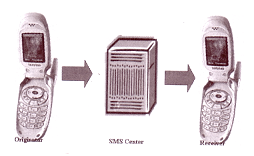
\includegraphics{gambar/gambar1}
    \caption{Skema cara kerja SMS}
    \label{kerja SMS}
\end{figure}

Sebuah SMSC biasanya didesain untuk dapat menangani  sort message dari berbagai sumber seperti Voice Mail System (VMS), Web-based messaging, e-mail Integration, Eksternal Short Messaging Entitas (ESME), dan lain-lain. Dalam interkoneksi dengan entitas dalam jaringan komunikasi wireless seperti Home Location Register (HLR) dan Mobile Switching Centre (MSC), SMSC biasanya selalu menggunakan Signal Transfer Point (STP).
	
Layanan SMS merupakan sebuah layanan yang bersifat non-real time dimana sebuah short message dapat di submit ke suatu tujuan, tidak peduli apakah tujuan tersebut aktif atau tidak. Bila dideteksi tujuan tidak aktif, maka sistem akan menunda pengiriman ke tujuan hingga tujuan aktif kembali. Pada dasarnya sistem SMS akan menjamin delivery dari suatu short message hingga sampai ke tujuan. Kegagalan pengiriman yang bersifat sementara seperti tujuan yang tidak diaktifkan selalu teridentifikasi sehingga pengiriman ulang short message akan selalu dilakukan kecuali bila diberlakukan aturan bahwa short message yang telah melampaui batas waktu tertentu harus dihapus dan dinyatakan gagal terkirim.
	
Karakteristik utama dari SMS adalah SMS merupakan sebuah sistem pengiriman data dalam paket dengan bandwidh kecil. Dengan karakteristik ini, pengiriman suatu data yang pendek dapat dilakukan dengan efisensi yang sangat tinggi. Pada awalnya SMS diciptakan untuk menggantikan layanan paging dengan menyediakan layanan serupa yang bersifat two-way messaging ditambah dengan notification service, khususnya untuk voice mail. Pada perkembangan selanjutnya, muncul jenis-jenis layanan lain seperti mail, fax, dan paging integration, interactive banking, information service, dan integrasi dengan aplikasi berbasis internet. Selain itu juga berkembang layanan wireless seperti SIM download for active action, debet dan profile editing, Wireless Point of Sale (POSs), serta layanan aplikasi lapangan seperti remote reasing, remote sensing, dan Location Base Services (LBS). Integrasi dengan aplikai berbasis internet mendorong timbulnya layanan seperti web-based messaging, gaming dan chatting.
	
Pada era kopetensi global saat ini, perbedaan layanan merupakan faktor yang cukup signifikan untuk mencapai sukses service provider. Sekali sebuah layanan tergelar seperti telepon, maka  SMS merupakan sebuah senjata yang cukup ampuh dalam rangka diferensiasi layanan. Bahkan jika pasar menerima dengan antusias, maka tidak mustahil SMS akan menjadi sumber pendapatan baru bagi service provider atau operator telekomunikasi.
	
\section{Arsitektur dan Elemen Jaringan SMS}
Untuk implementasi layanan SMS, operator menyediakan apa yang disebut sebagai SMS Centre(SMSC). Secara fisik SMSC dapat berwujud sebuah PC biasanya mempunyai interkonektivitas  dengan jaringan GSM. Salah satu implementasi SMSC Open Source adalah Kannel, yang digunakan untuk membangun WAP dan SMS Gateway. SMSC secara operasional dapat pula terkoneksi dengan jaringan TCP/IP, sehingga dapat dibangun berbagai aplikasi internet  yang mempunyai hubungan dengan jaringan GSM, sebagai contoh e-mail to SMS, SMS calender remainder, dan sebagainya. 

Layanan SMS dibangun dari berbagai entitas yang saling terkait dan mempunyai fungsi dan tugas masing-masing. Tidak ada satu pun dalam sistem SMS yang dapat bekerja secara parsial. Entitas dalam jaringan SMS ini disebut juga elemen jaringan SMS. Secara umum arsitektur sistem SMS, khususnya untuk sistem yang diintegrasikan dengan jaringan wireless, adalah sebagai berikut: 

\begin{figure}[ht!]
  \centering
    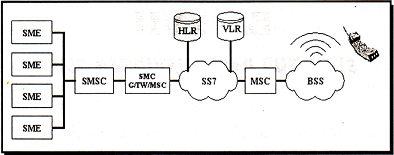
\includegraphics{gambar/gambar5}
    \caption{Arsitektur dasar jaringan SMS}
    \label{jaringan SMS}
\end{figure}

Dari gambar arsitektur dasar SMS, di sebelah kiri dapat dilihat SMSC memiliki interkonektivitas dengan SME (Short Messeging Entity) yang dapat berupa jaringan e-mail, web, dan voice e-mail. SMSC inilah yang akan melakukan manajemen pesan SMS, baik untuk pengiriman, pengaturan antrian SMS, ataupun penerimaan SMS.

\subsection{External Short Message Entities}
Dapat dikatakan bahwa Short Message Entity (SME) merupakan entitas dalam sistem 	SMS yang dapat berada pada jaringan, berupa perangkat bergerak, atau merupakan service centre yang berada diluar jaringan. ESME sendiri, sesuai dengan namanya, merupakan sebuah SME yang berada di luar jaringan SMS. Saat ini sebagian besar ESME berada pada jaringan data seperti jaringan TCP/IP yang didalamnya  termasuk internet. Beberapa macam ESME di antaranya adalah :

\textbf{1.	Voice Mail System}
Voice Mail System (VMS) merupakan perangkat yang berfungsi untuk menerima, menyimpan dan menjalankan voice message, ditujukan untuk pelanggan yang sedang sibuk dan sedang tidak dapat dihubungi melalui sambungan voice.

\textbf{2.	Web}
Web merupakan sebuah layanan yang sangat populer pada jaringan data terutama internet. Pesatnya perkembangan internet dengan jumlah pertumbuhan penggunanya yang juga sangat tinggi, membuat internet sebagai sebuah entitas dalam sistem SMS yang banyak membangkitkan tarif SMS.

\textbf{3.	E-mail}
E-mail merupakan salah satu layanan yang paling banyak digunakan dalam internet. SMS harus dapat mendukung interkoneksi dengan teknologi e-mail. Untuk itu kemudian muncul layanan yang juga cukup banyak digemari, yaitu email-to-sms dan sms-to-email.

\subsection{Short Message Service Centre}
Terminologi Short Message Service Centre (SMSC) mengacu pada suatu yang berupa hardware dan software. SMSC merupkan sebuah entitas yang bertanggung jawab untuk memperkuat, menyimpan, dan meneruskan short message dari satu titik ke titik lain yang merupakan tujuan , misalnya dari suatu SME ke perangkat telepon bergerak. 

Sebuah SMSC harus memiliki keandalan yang tinggi, kapasitas yang cukup dan throughout yang memadai dalam menangani short message. Selain itu, sistem harus bersifat fleksibel dan terukur agar dapat mengakomodasi pertumbuhan permintaan layanan  SMS. Faktor lain yang juga harus diperhatikan adalah aplikasi harus dapat dioperasikan dengan mudah, begitu juga pemeliharaannya. Sebagai contoh adalah fleksibilitas untuk aktifitas layanan baru dan upgrade software.

SMSC juga dapat digunakan untuk mengirim data biner yang dapat diinterpretasikan oleh piranti bergerak tanpa ditampilkan kepada pengguna. Kemampuan ini memungkinkan operator mengatur pelanggannya dengan menyediakan mekanisme untuk memprogram piranti bergerak milik para pelanggan.

Contoh dari pelayanan semacam ini adalah pemrograman piranti bergerak yang memungkinkan profil pelanggan dan karakteristik berlangganannya di-download ke piranti bergerak  (pelanggan dapat diaktifkan/dinonaktifkan berdasarkan data yang telah di download) dan davice of change yang memungkinkan digunakannya SMS untuk melaporakan biaya yang timbul dari pemakaian telepon si pelanggan. Salah satu metode yang menarik untuk memberikan coustomer support adalah dengan menawarkan daftar jawaban terhadap Frequently Asked Questions (FAQ) melalui pesan pendek SMS juga dapat digunakan untuk mengingatkan para pelanggan  akan pembayaran yang jatuh tempo. Cara ini tentunya dapat mengurangi biaya dan menjamin sampainya pesan tersebut secara tepat waktu.

\subsection{SMS-Gateway dan SMS-Interworking}
SMS Gateway Mobile Switching Centre (SMS-GMSC) adalah sebuah apliksi MSC yang mampu menerima pesan singkat dari SMSC, mengintrogasi Home Locator Register (HLR) untuk informasi routing, dan mengirimkan pesan-pesan pendek tersebut ke MSC dari piranti yang bergerak yang dituju.

SMS Interworking Mobile Switching Centre (SMS-IWMSC) adalah aplikasi MSC yang mampu menerima pesan pendek dari jaringan bergerak dan mengirimnya ke SMSC yang tepat. SMS-GMSC/SMS-IWMSC biasanya terintegrasi dengan SMSC.

\subsection{Signaling System 7}
Signaling System 7 (SS7) merupakan protokol komunikasi yang digunakan untuk menghubungkan Short Message Service Centre (SMSC) dengan Mobile Switching Centre (MSC), SS7 juga  digunakan untuk menghubungkan ke lebih dari satu elemen  jaringan yang lain.

\subsection{Home Locator Register}
Home Locator Register (HLR) adalah basis data yang digunakan untuk penyimpanan permanen, pengelolaan langganan dan profil layanan. Ketika diinterogasi oleh SMSC, HLR memberikan informasi routing mengenai pelanggan yang ingin dituju.

HLR juga dapat memberitahu SMSC, yang sebelumya mengalami kegagalan dalam pengiriman pesan pendek  ke piranti bergerak tertentu, bahwa sekarang piranti mobile tersebut telah dikenali oleh jaringan bergerak, dan dengan demikian pesan telah dapat dikirim.

\subsection{Mobile Switching Centre}
Mobile Switching Centre (MSC) merupakan fungsi penyaklaran sistem dan pengendalian panggilan ke dan dari sistem telepon dan data yang lain. MSC akan mengirimkan pesan pendek ke pelanggan tertentu melalui base station yang sesuai.

\subsection{Visitor Location Register}
Visitor Location Register (VLR) adalah basis data yang berisi informasi temporal mengenai pelanggan yang berasal dari suatu HLR yang roaming ke HLR lainnya. Informasi ini dibutuhkna oleh MSC untuk melayani pelanggan yang berkunjung.

\subsection{Base Station System}
Semua fungsi yang terkait dengan trasmisi sinyal radio elektromagnetis antara MSC dan piranti bergerak dilakukan di Base Stasion System (BSS). BSS terdiri dari Base System Controls (BSCs), dan Base Transceiver Stations (BTSs), juga dikenal dengan wilayah sel/sel.
BSC dapat mengendalikan satu atau lebih BTS dan bertanggung jawab dalam pemberian sumber data yang semestinya ketika pelanggan bergerak dari satu sektor suatu BTS ke sektor lain, terlepas apakah sektor  berikutnya tersebut berada dalam BTS yang sama atau beda.

\section{Layanan Pesan Pendek}
Badan yang bertugas untuk menetukan standar layanan pesan pendek adalah European Telecommunication Standards Institute (ETSI) dan badan standar Amerika yaitu Telecommunication Industry Association (TIA) telah menetapkan standar dari Mobile Application Part (MAP) yang menggunakan layanan dari system pensinyalan no.7 pada bagian kemampuan transaksinya. MAP yang bertugas mendefinisikan operasi yang dibutuhkan untuk mendukung layanan pesan pendek tersebut oleh ESTI ditetapkan sebagai standar yang dikenal dengan sebutan GSM-MAP sedangkan TIA menetapkan setandar  sebagai IS-41. Adapun operasi dari MAP yang diperlukan untuk membentuk layanan pesan pendek secara Pont-to-Point adalah sebagai berikut:
\textbf{1.	Routing Information Request}
Sebelum mencoba mengirim pesan pendek, SMSC harus mengambil informasi routing untuk menentukan MSC mana yang melayani piranti bergerak yang sedang dituju. Hal ini dilakukan dengan mengintrogasi HLR dengan menggunakan  mekanisme SMS request dan send routing info for short msg.

\textbf{2.	Pengiriman Pesan Pendek Point-to-Point}
Mekanisme ini memungkinkan SMSC mengirim pesan pendek ke MSC yang sedang melayani piranti bergerak yang dituju dan mencoba mengirimkan pesan ke MS, kapan saja MS itu terdaftar, bahkan ketika MS sedang melakukan panggilan suara atau data. Operasi pengiriman pesan pendek memberikan layanan pengiriman yang terkonfirmasi.
Operasi ini bekerja sama dengan subsistem base station ketika pesan sendang dikirim dari MSC ke MS. Oleh karena itu, hasil dari opersi tersebut bisa berhasil bisa juga gagal. Pingiriman pesan pendek Point-to-Point dilakukan dengan menggunakan mekanisme short message delevary Point-to-Point/SMD-PP dan forward short message.

\textbf{3.	Indikasi Penangguhan Pesan Pendek}
Operasi ini diaktifkan ketika usaha pengiriman pesan pendek oleh SMSC gagal karena memberikan kesempatan bagi SMSC untuk meminta HLR menambahkan alamat SMSC ke dalam daftar SMSC yang akan diberitahu ketika piranti bergerak yang dituju tadi telah dapat dihubungi.
Indikasi penangguhan pesan pendek ini direalisasikan melalui penggunaan mekanisme SMS notification indicator dan send messsage waiting data.

\textbf{4.	Notifikasi Service Centre}
Operasi ini memungkinkan HLR menginformasikan SMSC, yang sebelumnya mengalami kegagalan dalam usaha pengiriman pesan pendek ke piranti bergerak tertentu, bahwa piranti bergerak tersebut sekarang telah dapat diakses oleh jaringan bergerak. Notifikasi service Centre ini dicapai dengan menggunakan mekanisme SMS notification dan alert service

\subsection{Elemen Layanan}
SMS terdiri dari elemen layanan yang relevan terhadap penerimaan dan pengiriman pesan pendek, yaitu :

\textbf{1.	Message Expiration}
SMSC akan menyimpan dan mencoba mengirim kembali pesan yang mengalami kegagalan, sampai pengiriman tersebut berhasil atau sampai batas waktu yang ditentukan per pesan atau per platform telah tiba.

\textbf{2.	Priority}
Merupakan elemen informasi yang disediakan oleh SME untuk memberi tanda pesan-pesan yang penting dan membedakannya dari pesan yang biasa. Pesan penting biasanya lebih diprioritaskan daripada pesan biasa, terlepas dari waktu kedatangan pesan tersebut ke platform SMSC. SMS juaga meyediakan time stamp yang menyatakan waktu pengiriman pesan ke SMSC dan memberikan suatu petunjuk pada handset mengenai masih ada atau tidaknya pesan yang akan dikirim.

\subsection{Layanan Pelanggan}

	Sistem SMS memiliki dua layanan Point-to-Point bagi pelanggan, yaitu:
	
\textbf{a.	Mobile Originated Short Message}
Mobile Originated (MO) Short Messages dikirim dari handset yang MO-capable ke SMSC dan dapat ditujukan ke palanggan bergerak lainnya atau pada pelanggan di jaringan fixed seperti jaringan Internet Protokol (IP). 
Mobile Termenated (MT) Short Messages dikirim dari SMSC ke handset dan dapat sampai ke SMSC dari pelanggan bergerak  yang lain melalui MO-SM atau sumber lain seperti sistem voce-mail atau operator.
Pada layanan MO-SM selalu ada laporan yang dikirimkan ke hendset, baik yang menginformasikan kegagalan pengiriman  dan mengidentifikasi penyebabnya. 

\textbf{b.	Mobile Terminated Short Message}
Untuk MT-SM, juga selalu ada laporan yang diberikan kepada SMSC yang isinya bisa berupa konfirmasi pengiriman pesan pendek ke handset maupun informasi kegagalan pengiriman pesan dan mengidentifikasi penyebab kegagalan tersebut.

\section{Aplikasi Berbasis SMS}\
Aplikasi berbasis SMS, tergantung dari metode akses dan enkoding pada pembawa data, layanan pesan pendek Point-to-Point dapat mengirimkan sampai 190 karakter ke suatu Short Message Entity (SME).

Untuk pesan yang segera dikirim, hanya dilakukan satu kali pengiriman untuk setiap permintaan pelayanan. Untuk pesan yang tidak membutuhkan pengiriman dengan segera, dapat dilakukan satu kali atau lebih pengiriman, sampai acknowledgment diterima.

Dalam jaringan GSM, jenis layanan pesan diidentifikasikan dengan Protocol Identifier Information Element, yang membedakan antara protokol tingkat tinggi atau interworking yang sedang digunakan, Misalnya telex , dan telepon suara.

Banyak aplikasi layanan yang dapat diimplementasikan dengan mengkombinasikan elemen-elemen layanan SMS. Disamping layanan notifikasi yang sudah jelas ada, SMS juga dapat digunakan dalam layanan satu arah atau layanan interaktif yang memungkinkan akses nirkabel ke semua jenis informasi dimanapun berada.

Dengan memanfaatkan berbagai teknologi baru yang menggabungkan browser, server, dan markup language yang didesain untuk perangkat bergerak, SMS memungkinkan piranti nirkabel untuk mengakses dan mengirimkan informasi secara aman dari internet atau intranet dengan cepat dan efisien. Salah satu dari teknologi tersebut dimana SMS dapat memberikan suatu pendekatan yang kooperatif adalah WAP, yang memungkinkan pengiriman data bagi para pengguna piranti bergerak nirkabel.

%-------------------------------------------------------------------------------
\chapter{ANALISIS DAN PERANCANGAN}

\section{Analisis}
Penyajian informasi sedemikian rupa sehingga dapat diakses tanpa dibatasi oleh ruang dan waktu dengan memanfaatkan teknologi yang ada. Hal tersebut harus dibarengi dengan kemudahan dalam pengoperasian dan biaya yang relatif murah.

Harus dipastikan bahwa sistem layanan informasi ini dapat berjalan dengan baik. Disamping itu, juga perlu dipastikan tentang orang yang akan mengoperasikan, mengontrol dan memelihara sistem tersebut.

Analisis masalah yang dilakukan oleh penulis adalah analisis yang difokuskan pada Pusat Informasi. Berikut ini akan dijelaskan rincian layanan yang berhasil penulis analisis.

\textbf{1.	Informasi Jadwal Shalat}
Menampilkan informasi jadwal shalat berdasarkan kota, bulan dan tanggal. Input yang berupa bulan dan tanggal kemudian di ubah dan disesuaikan dengan ID jadwal shalat. Jadwal shalat yang menjadi acuan adalah jadwal shalat untuk Kota Jakarta, sedangkan jadwal shalat untuk kota-kota lainnya menyesuaikan (penambahan dan pengurangan) dengan jadwal shalat Kota Jakarta.
Berikut ini struktur data tabel jadwal shalat, tabel ini mempunyai enam elemen data yaitu: tanggal dan lima waktu shalat wajib dalam sehari (jadwal shalat Kota Jakarta).

Tanggal pada tabel tersebut hanya terdiri dari bulan dan tanggal, sedangkan tahun tidak diikut sertakan. Untuk waktu jadwal shalat terdiri dari jam dan menit. Misalnya waktu shalat shubuh pada tabel diatas (04.30) berarti pukul 04.00 lewat/lebih 30 menit.

Untuk penyesuaian jadwal-shalat kota-kota selain Kota Jakarta maka diperlukan tabel lagi yang berupa tabel penyesuaian yang terdiri dari dua elemen data, yaitu nama kota dan parameter peyesuaian. Parameter penyesuaian berupa angka (menit) penambah atau pengurang terhadap waktu jadwal shalat Kota Jakarta. 


\textbf{2.	Informasi Arah Kiblat}
Menampilkan Informasi Arah Kiblat berdasarkan kota. Dimana perhitungan untuk menentukan arah kiblat tersebut menghitung posisi kota tersebut pada garis lintang dan bujur tertentu terhadap posisi garis lintang dan bujur Kota Mekkah (Ka’bah) berada.
Struktur data tabel arah kiblat tersebut terdiri dari dua elemen data, yaitu kode kota dan arah kiblat. 
untuk kota kota merupakan tiga huruf singkatan dari nama kota tersebut, misalnya BDG merupakan singkatan dari Bandung. Sedangkan untuk arah kiblat (64,50), angka tersebut adalah derajat dalam format desimal bukan dalam format koordinat waktu (64˚ 50’).
Selain Informasi arah kiblat berdasarkan input kode kota yang merupakan singkatan dari nama kota tertentu. Informasi arah kiblat dapat juga diperoleh dengan input koordinat posisi pada permukaan bumi. Koordinat tersebut adalah koordinat pada garis lintang dan bujur. Koordinat tersebut didapat dengan alat GPS (Global Position System).
Sedangkan perhitungannya menggunakan rumus matematika yang dipaparkan oleh Dr. Mohibullah N. Durrani, yang merupakan koordinator bidang informasi astronomi Islamic Society of  North America (ISNA). Dengan menggunakan perhitungan ini maka kita dapat menghitung arah kiblat dari tempat di seluruh dunia dengan berbasis pada garis lintang dan garis bujur.

\section{Perancangan}
Merancang arsitektur pada awal pembangunan suatu sistem adalah suatu hal yang sangat penting. Dengan merancang arsitektur, suatu sistem yang dibentuk akan memiliki konstruksi yang baik, proses pengolahan data yang tepat dan akurat, bernilai, memiliki aspek user friendly dan memiliki dasar-dasar untuk pengembangan selanjutnya. Dalam hal ini, seorang pemrogram harus dapat menentukan modul-modul yang dapat diperlukan, dan selain itu, pembuat sistem harus dapat menjalankan strategi  untuk menangani kesalahan dan memperhitungkan pengembangan yang mungkin terjadi.
Pada saat merancang arsitektur program, penyusun harus dapat merinci format input dan output serta prosedur yang efektif, struktur data dan teknik yang akan digunakan, manajemen memori, penanganan kesalahan, mendefinisikan fungsi-fungsi yang disediakan. Sementara itu untuk pemrograman berorientasi objek, penyusun harus dapat merinci objek utama yang diimplementasikan.  
Setelah proses perancangan arsitektur program ini selesai, maka pemrogram dapat mulai menyusun suatu algoritma yang dibuat dengan tujuan untuk menyelesaikan persoalan yang ada.
Algoritma tersebut tidak dibuat sekali jadi. Oleh karena itu perlu selalu dikaji secara terus-menerus, sehingga diperoleh suatu algoritma yang lengkap, tepat, benar dan relevan.
Algoritma yang sudah disusun  juga perlu dikoreksi lagi, jika terdapat kesalahan maka harus dilakukan revisi. Menyusun algoritma  sama dengan menulis langkah-langkah dari persoalan yang ada. Algoritma harus memiliki kebenaran secara logika, sehingga setelah langkah-langkah revisi selesai, maka harus dilakukan pengecekan logika sebelum siap untuk diimplementasikan. Berikut ini adalah algoritma yang disajikan dalam bentuk flowchart, yaitu:

\begin{figure}[ht!]
  \centering
    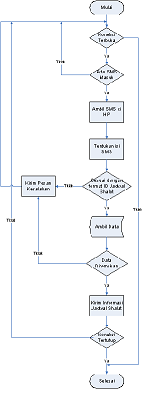
\includegraphics{gambar/gambar3}
    \caption{Diagram Alir Program untuk permintaan Jadwal Shalat}
    \label{flowchart}
\end{figure}

Dari diagram alir diatas, setelah program dijalankan, program akan melakukan koneksi dengan SMS Gateway. Program akan mengecek apabila ada yang melakukan permintaan informasi jadwal shalat (ada SMS masuk), maka program akan mengambil SMS tersebut dan kemudian melakukan validasi terhadap SMS tersebut sesuai dengan format yang telah ditentukan. Apabila format sesuai maka akan diteruskan dengan mengecek apakah data tersebut ada dalam basis data, apabila data tidak ditemukan pada basis data maka akan dilakukan pengiriman bahwa data tidak diketemukan. Sedangkan apabila data ditemukan maka akan dilakukan pengiriman pesan informasi yang diminta ke nomor ponsel yang melakukan permintaan informasi tersebut.

\begin{figure}[ht!]
  \centering
    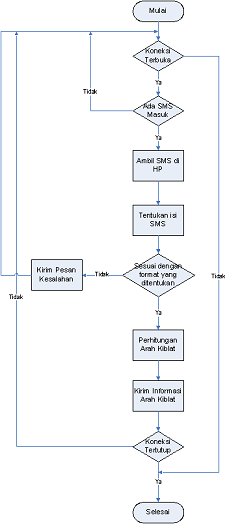
\includegraphics{gambar/gambar4}
    \caption{Diagram Alir Program untuk permintaan Arah Kiblat}
    \label{kripto}
\end{figure}




%-----------------------------------------------------------------
%Disini akhir masukan Bab
%-----------------------------------------------------------------

%-----------------------------------------------------------------
%Disini awal masukan untuk Daftar Pustaka
%-----------------------------------------------------------------
%%\nocite{Abel2010,Guerbas201350}
%%\bibliography{research-plan}
%%\bibliographystyle{plainnat}
\begin{thebibliography}{9}

\bibitem[satu(2000)]{satu01}
Budicahyanto, Dwi. 2004. Membangun Aplikasi Handphone dengan FBUS dan
Visual Basic. Yogyakarta: Andi Offset.


\bibitem[dua(2003)]{dua02}
Imron, Romzi R. 2004. Membuat Sendiri SMS Gateway (ESME) Berbasis Protokol
SMPP. Yogyakarta: Andi Offset

\bibitem[tiga(2004)]{tiga03}
Khang, Bustam. 2002. Trik Pemrograman Aplikasi Berbasis SMS. Jakarta: PT. Elex
Media Komputindo.

\bibitem[empat(2013)]{empat04}
Sutedjo, Budi, Dharma O dan Handoko, Yosia. 2003. Teleakses Database Pendidikan
Berbasis Ponsel. Yogyakarta: Andi Offset.


\end{thebibliography}
\addcontentsline{toc}{chapter}{DAFTAR PUSTAKA}
%-----------------------------------------------------------------
%Disini akhir masukan Daftar Pustaka
%-----------------------------------------------------------------

\end{document}
